\documentclass[10pt,foldmark,notumble]{leaflet}
\renewcommand*\foldmarkrule{.3mm}
\renewcommand*\foldmarklength{5mm}

\usepackage{amsmath}
\usepackage[utf8]{inputenc}
\usepackage[T1]{fontenc}
\usepackage{textcomp}
\usepackage{mathptmx}
\usepackage[scaled=0.9]{helvet}
\makeatletter
\def\ptmTeX{T\kern-.1667em\lower.5ex\hbox{E}\kern-.075emX\@}
\DeclareRobustCommand{\ptmLaTeX}{L\kern-.3em
        {\setbox0\hbox{T}%
         %\vb@xt@ % :-)
         \vbox to\ht0{\hbox{%
                            \csname S@\f@size\endcsname
                            \fontsize\sf@size\z@
                            \math@fontsfalse\selectfont
                            A}%
                      \vss}%
        }%
        \kern-.12em
        \ptmTeX}
\makeatother
\let\TeX=\ptmTeX
\let\LaTeX=\ptmLaTeX
\usepackage{shortvrb}
\MakeShortVerb{\|}
\usepackage{url}
\usepackage{graphicx}
\usepackage[dvipsnames,usenames]{color}
\definecolor{LIGHTGRAY}{gray}{.9}
\definecolor{LIGHTBLUE}{rgb}{0.2,0.2,0.5}

%%%%\renewcommand{\descfont}{\normalfont}
\newcommand\Lpack[1]{\textsf{#1}}
\newcommand\Lclass[1]{\textsf{#1}}
\newcommand\Lopt[1]{\texttt{#1}}
\newcommand\Lprog[1]{\textit{#1}}

\newcommand*\defaultmarker{\textsuperscript\textasteriskcentered}

%%%%%%%%%%%%%%%%%%%%%%%%%%%%%%%%%%%%%%%%%%%%%%%%%%%%%%%%%%%%%%%%%%%%%%%%%%%%%%

\title{\bf LuXeria}

\author{%
\Large \bf Zentralschweizer\\\bf OpenSource Verein
}
\date{\bf 5. Februar, 2012 }

%\CutLine*{1}% Dotted line without scissors
%\CutLine{6}%  Dotted line with scissors

%\AddToBackground{1}{%  Background of a small page
%  \put(0,0){\textcolor{Cerulean}{\rule{\paperwidth}{\paperheight}}}}

%\AddToBackground{1}{%  Background of a small page
%  \put(35,200){
\includegraphics[scale=1]{../lux_logo.pdf}}}

\AddToBackground{6}{%  Background of a small page
  \put(0,0){\textcolor{LIGHTBLUE}{\rule{\paperwidth}{\paperheight}}}}


\AddToBackground*{2}{% Background of a large page
  \put(\LenToUnit{.5\paperwidth},\LenToUnit{.5\paperheight}){%
    \makebox(0,0)[c]{%
      \resizebox{.9\paperwidth}{!}{\rotatebox{35.26}{%
        \textsf{\textbf{\textcolor{LIGHTGRAY}{LuXeria}}}}}}}}


\usepackage[ngerman]{babel}
\usepackage{lipsum}
\usepackage{url}


\begin{document}
\pagenumbering{gobble}
\clearpage
\thispagestyle{empty}
\maketitle

\vfill
\begin{figure}
\centering

\includegraphics[width=0.8\textwidth]{../lux_logo.pdf}
\end{figure}


\newpage
\section{LuXeria}
LuXeria ist ein Verein im Raum Luzern, welcher zum Ziel hat 
quelloffene Systeme und Applikationen zu fördern.


Der Verein wurde gegründet um die Entschlossenheit gegenüber
FreeSoftware bzw. OpenSource zu unterstreichen und nicht einfach 
nur als User-Group von Linux Anwendern und Programmierern wahrgenommen
zu werden.

\subsection{Motto}
Das Motto des Vereins lautet \emph{OpenSource -- Open Mind}.
Die Mitglieder von LuXeria vertreten die Meinung, dass 
FreeSoftware bzw. OpenSource wichtig ist und der Austausch 
unter den Usern im Zentrum stehen soll. 

\subsection{Mitglieder}
Die Mitglieder der LuXeria kommen aus allen Schichten der Gesellschaft.
Vom Lehrling, Quereinsteiger bis zum alten Hasen der IT ist so ziemlich 
alles vertreten. Die Meisten der Mitglieder sind jedoch Studenten der 
Informatik im Raum Zentralschweiz (Hochschule Luzern, Hochschule 
Rapperswil, Eidgenössische Technische Hochschule). 
Aktuell ist die LuXeria mit 15 Mitglieder vertreten.

Zentraler Bestandteil und gemeinsamer Nenner der meisten 
Mitglieder ist Linux. Besondere Programme oder Programmierspachen 
sind sehr individuell vertreten.

\section{Treffen}
Jeweils am Mittwochabend treffen sich die Mitglieder von LuXeria 
im Vereinslokal und geniessen dort ein gemeinsames Abendessen.
An diesen Treffen findet der primäre Austausch statt, meist 
erfolgt dies in offenen Diskussionen oder kleineren Arbeitsgruppen
statt. In unregelmässigen Intervallen finden spontane oder
angekündigte Präsentationen, Vorträge und Demos statt.

\subsection{Events}
LuXeria versteht sich nicht nur als ein Zweckorientierter 
Verein sondern auch als soziale Gruppe. So finden ab und
zu auch vom Verein unabhängige Treffen und Events statt.

\section{Angebote}
\subsection{Bibliothek}
LuXeria verfügt über eine Buchsammlung die sich dank 
grosszügiger Spenden sehr ausgeweitet hat.
Der Grossteil der Bücher und Magazine ist klar im
Bereich der Programmierung und Systeme angesiedelt.

\subsection{Chat}
LuXeria betreibt einen IRC Channel auf freenode. Dieser
bietet den Mitgliedern und auch Interessierten direkten
Zugang und Austauschmöglihckeiten. Siehe
\url{chat.freenode.net} -- \url{#luxeria}

\subsection{Infrastruktur}
LuXeria nutzt die Räumlichkeiten des VFI (Verein zur 
Förderung der ICT-Berufsbildung) und hat somit Zugang 
zu einer sehr guten Infrastruktur wie etwa modernen
Schulungsräumen oder Racks.

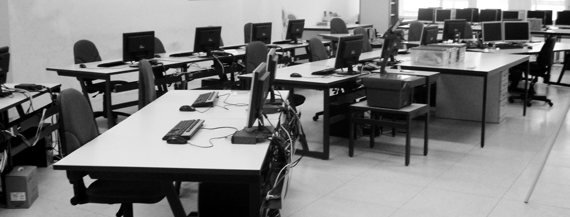
\includegraphics[width=1\textwidth]{kursraum.jpg}

\subsection{Elektronik Labor}
LuXeria betreibt ein relativ kleines aber gut
ausgerüstetes Elektronik Labor. Zur Grundausrüstung 
des Labors gehören Lötstationen, digitale und analoge
Oszilloskope, Logik-Analyser, Linearnetzteile und eine
kleine Komponentensammlung.

\section{Mitgliedschaft}
LuXeria hat keine speziellen Aufnahmebedingungen und 
Einschränkeungen wie Alter oder Fachbereich. Jeder der
sich mit dem Verein identifizieren kann ist herzlich 
willkommen. Der Verein unterscheidet aber die Mitglieder
in Aktiv-, Passiv-, Ehrenmitglieder und Gönner.

Eine Mitgliedschaft wird formell durch den jährlichen 
Mitgliederbeitrag bestätigt. 

\section{Finanzen}
Der Verein hat nebst den Mitgliederbeiträgen kein
regelmässigen Einkommen und besitzt auch keine
Finanz-Strategie. 

Spenden erfährt der Verein meist in Form von IT-
Material, Literatur oder Einladungen zu Messen
und anderen Veranstatlungen.

\section{Lage}
LuXeria hat sein Lokal in den Räumen des VFI 
und somit in Adligenswil innerhalb des Areals 
der Ringier Print. Besucher sind desshalb angeweisen
eine vorgängige Anmeldung zu tätigen. 

Das Lokal ist per ÖV gut erreichbar und liegt lediglich 
ca. 10 Minuten von Luzern entfernt (Postauto, Linie 73).

\newpage

\section{Kontakt}
Der Verein ist gegen aussen durch den Vorstand vertreten
und der Vereinspräsident ist der erste Ansprechpartner
für Fragen und Anregungen.

\begin{table}[h!]
        \begin{tabular}{l}
        LuXeria \\
        Ebikonerstrasse 75 \\
        6048 Adligenswil \\
        +41/76-371-12-89 \\
        info@luxeria.ch 
        \end{tabular}
\end{table}

\section{Lage}
\begin{figure}[h!]
\centering
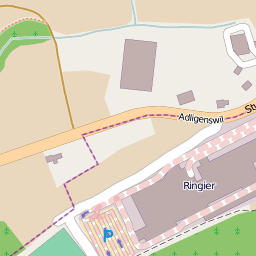
\includegraphics[width=0.8\textwidth]{lux_lage.png}
\end{figure}

\section{Vorstand}
\begin{table}[h!]
        \begin{tabular}{ll}
        Präsident       & Ervin Mazlagi\'c\\
        Vizepräsident   & Michael Zihlmann\\
        Kassier         & Freddy Ringier\\
        Aktuar          & Steve Ineichen 
        \end{tabular}
\end{table}

\end{document}
